\documentclass{article}

\usepackage[utf8]{inputenc}
\usepackage{caption}
\usepackage{csquotes}
\usepackage{multicol}
\usepackage{enumerate}
\usepackage{float}
\usepackage{graphicx}
\usepackage{mathtools}
\usepackage{pgfplots}
\usepackage{subcaption}
\usepackage{tikz}
\usepackage[a4paper, total={6in, 8in}]{geometry}

% Remove References from BibTeX heading
\usepackage{etoolbox}
\patchcmd{\thebibliography}{\section*{\refname}}{}{}{}

% Path for images
\graphicspath{ {./images/} }


\setlength\parindent{0pt}


\title{
    Parameterising Temperature and Cooling Rate \\
    \large for Simulated Annealing applied to the \\
    Travelling Salesman Problem
}

\author{Gary Sun}

\date{2021}

\begin{document}

\maketitle

\begin{abstract}
    In this paper, we explore the impact of different values of initial temperatures and cooling rates for Simulated Annealing.
    These values are bench marked using the Travelling Salesman Problem, to determine the impact of the values for different inputs. 
    Finally, we determine if there is a correlation between the ideal initial temperature and cooling rate with the given problem model, and subsequently a way to parameterise the temperature and cooling rate based off the input.
\end{abstract}

\tableofcontents

%%%%%%%%%%%%%%%%%%%%%%%%%%%%%%%%%%%%%%%%%%%%%%%%%%%%%%%%%%%%%%%%%%%%%%%%%%%%%%%%
\newpage
\section{Introduction}
\subsection{The Travelling Salesman Problem}
The travelling salesman is an example of an NP-hard combinatorial optimisation problem.

It goes as follows:
\begin{quote}
Given a weighted graph, starting at a vertex, find the minimal cost to travel to all the vertices of the graph once, before returning back to the starting vertex.
\end{quote}

It has many applications, both in practise and theory i.e. in logistics (determining an optimal route of least cost), job scheduling (determine the best way to schedule a series of jobs on a set of machines) and also for bench marking optimisation algorithms
\\

The specific purpose of this project is to explore the "Symmetric" Travelling Salesman Problem, where it is an undirected graph, i.e. there is no direction in the graph.
Whilst this halves the number of solutions as compared to the asymmetric TSP, it still has a super-polynomial running time as the number of solutions for $n$ cities is $(n - 1)! / 2$.

\begin{figure}[h]
    \centering
    \begin{tabular}{ |c|c| } 
        \hline
        City Count & Path Configurations \\ 
        \hline
        3 & 1 \\
        \hline
        5 & 12 \\
        \hline
        10 & $1.81 \times 10^{4}$ \\ 
        \hline
        20 & $6.08 \times 10^{16}$ \\
        \hline
        30 & $4.42 \times 10^{30}$ \\
        \hline
    \end{tabular}
    \caption{Number of path configurations per number of cities}
\end{figure}

\subsection{Algorithms for the Travelling Salesman Problem}

Due to the difficult nature of solving the TSP, there are two main categories of algorithms.

\begin{itemize}
    \item Exact algorithms
    \item Approximate algorithms
\end{itemize}

Exact algorithms have the benefit that they are able to find the optimal solution.
For example, the current record for the largest TSP problem is 85 900 cities which was solved using an ILP formulation \cite{cook12}.
However, they suffer from a longer runtime. \\

On the other hand approximate algorithms may be find a near optimal, whilst running relatively quickly \cite{helsgaun98}.
Hence, in practise, if the optimal is not required, it is suitable to use an approximate algorithm.
An example of common algorithm which can be applied for finding approximate solutions for TSP is Simulated Annealing.

%%%%%%%%%%%%%%%%%%%%%%%%%%%%%%%%%%%%%%%%%%%%%%%%%%%%%%%%%%%%%%%%%%%%%%%%%%%%%%%%
\newpage
\section{Simulated Annealing}
Simulated Annealing is a stochastic global search optimisation algorithm.
Whilst greedy searches may get stuck in a local minimum, Simulated Annealing aims to overcome this by probabilistically accepting worse options, and has a higher chance of finding the global minimum.
\\

\subsection{Origin}
It is based off annealing in metallurgy, where the structure of the material changes randomly rapidly. when the temperature is high.
As a result, at the beginning, SA may choose a solution, even if does not lead to an improvement in the objective function.
\\

However, overtime as the temperature drops and loses its internal energy, the structure settles into a more stable form.
Hence, as the temperature drops, the SA algorithm will with a higher probability discard solutions that do not improve the objective function, and always choosing those that improve the objective function.
\\

Finally, the resulting material structure reaches its absolute (global) minimum internal energy configuration.
Similarly, the SA algorithm will then find an approximate (or the) solution for maximising the objective function.
\\

Note the temperature and cooling rate has to be carefully selected.
If the temperature cools too fast, then in the process may get stuck at a local minimum. 
This is similar to what happens in a greedy method, where the search gets stuck in a local minimum.
Hence, the introduction of the temperature, and probabilistic acceptance of worse states allows for a higher chance of finding the global minimum.
\\

\subsection{Process}

\begin{enumerate}[Step 1:]
    \item Choose a suitable initial temperature $T_0$, cooling rate $r < 1$, a feasible solution $\mathbf{x}^{(0)}$, iteration counter $k = 0$, and the objective function $f$.
    \item Then select a neighbouring solution $\mathbf{x}^{(k + 1)}$ to $\mathbf{x^{(k)}}$, where $\mathbf{x}^{(k)}$ is the current solution at iteration $k$.
    \item Calculate  $\Delta f = f(\mathbf{x^{(k + 1)}}) - f(\mathbf{x^{(k)}})$. We then choose to take $\mathbf{x}^{(k + 1)}$ as the new solution with the following probability $P(\Delta f)$
    $$ P(\Delta f) = 
    \begin{dcases*}
        1 & if $\Delta f > 0$, \\
        \exp {\left( \frac{\Delta f}{T_k} \right)} & else
    \end{dcases*}
    $$
    \item If we have reached the max iterations, then stop
    \item Else, set $k = k + 1$, and $T_k = r T_k$, then go to Step 2
\end{enumerate}

\subsection{Temperature and Cooling Rate}

The initial temperature of the system determines how likely it is to accept worse solutions.
As shown in the selection function $\exp(\frac{\Delta f}{T})$ the temperature of the system should be proportional to the possible loss.
Hence, \textbf{the temperature should be proportional to how far apart the cities are} to retain the same probability of choosing a worse configuration.

\begin{figure}[H]
    \centering
    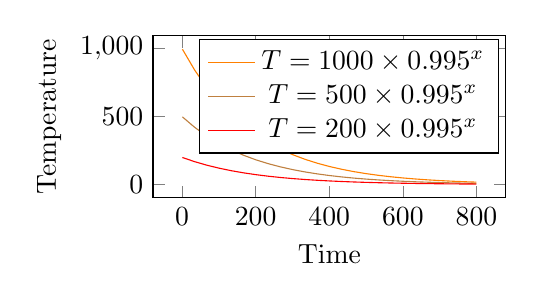
\begin{tikzpicture}
        \begin{axis}[
            width=0.5\textwidth,
            height=0.3\textwidth,
            xlabel=Time,
            ylabel=Temperature,
        ]
        \addplot[
            color=orange,
            domain=1:800
        ]
        {1000 * 0.995^x};
        \addlegendentry{$T = 1000 \times 0.995^x$}
        \addplot[
            color=brown,
            domain=1:800
        ]
        {500 * 0.995^x};
        \addlegendentry{$T = 500 \times 0.995^x$}
        \addplot[
            color=red,
            domain=1:800
        ]
        {200 * 0.995^x};
        \addlegendentry{$T = 200 \times 0.995^x$}
        \end{axis}
    \end{tikzpicture}
    \caption{Comparison of different initial temperatures}
\end{figure}


The cooling rate on the other hand determines the rate of change of the probability that we accept worse configurations.
\\

Whilst there are different cooling schedules, geometric cooling tends to perform well compared to other general methods \cite{cooling}.
This is due to high temperatures at the beginning allowing for more searching, whilst low temperatures later allows it to converge to a solution quickly.
\\

Ignoring other properties, denser materials cool slower.
If the TSP behaves like so, \textbf{the greater the number of cities, the slower the system should cool} as it is "denser".
Furthermore, if the number of cities is greater, there may also more local minimums, which can be mitigated by slower cooling.

\begin{figure}[H]
    \centering
    \begin{subfigure}[b]{0.48\textwidth}
        \centering
        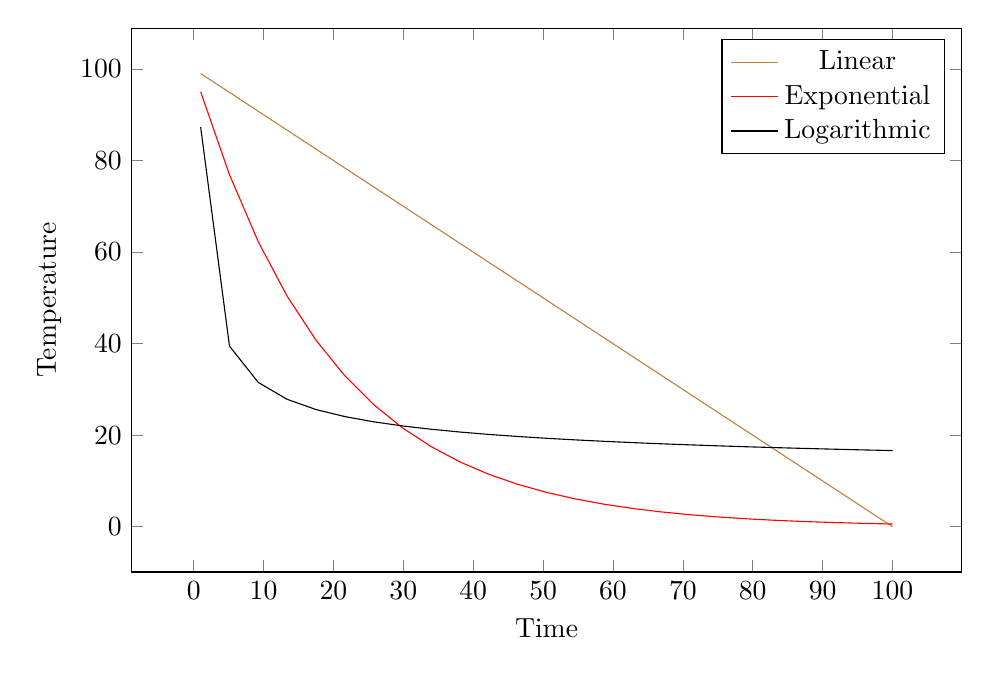
\begin{tikzpicture}
            \begin{axis}[
                xlabel=Time,
                ylabel=Temperature,
                width=1\textwidth,
                height=0.7\textwidth,
            ]
            \addplot[
                color=brown,
                domain=1:100
            ]
            {100 - x};
            \addlegendentry{Linear}
            \addplot[
                color=red,
                domain=1:100
            ]
            {100 * 0.95^x};
            \addlegendentry{Exponential}
            \addplot[
                color=black,
                domain=1:100
            ]
            {350/(1 + 10 * log10(1 + x))};
            \addlegendentry{Logarithmic}
            \end{axis}
        \end{tikzpicture}
        \caption{Comparison of different cooling schedules}
    \end{subfigure}
    \hfill
    \begin{subfigure}[b]{0.48\textwidth}
        \centering
        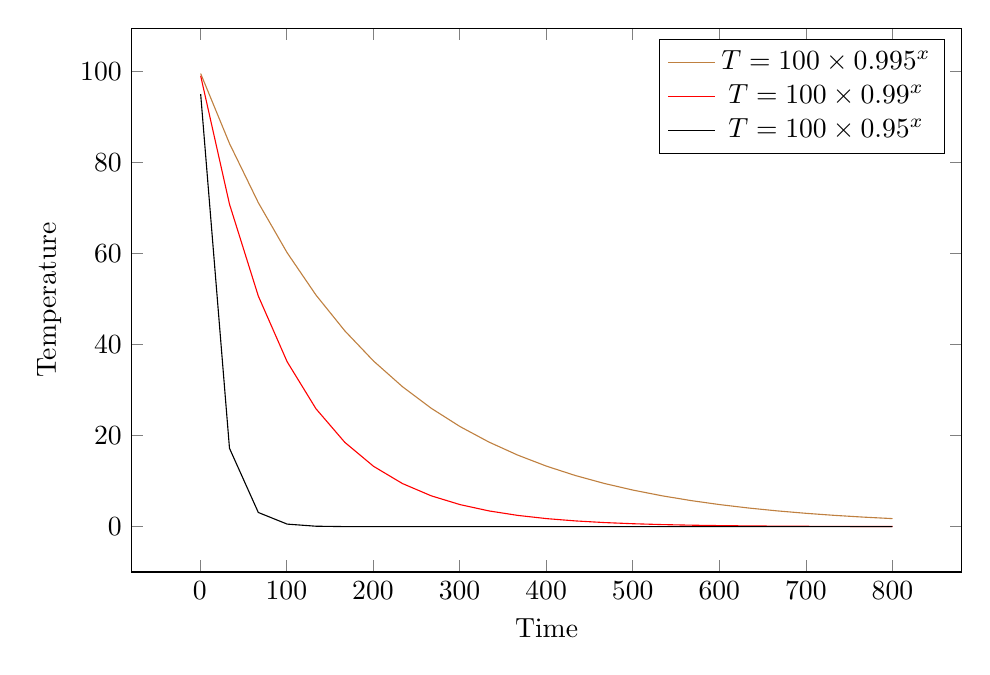
\begin{tikzpicture}
            \begin{axis}[
                xlabel=Time,
                ylabel=Temperature,
                width=1\textwidth,
                height=0.7\textwidth,
            ]
            \addplot[
                color=brown,
                domain=1:800
            ]
            {100 * 0.995^x};
            \addlegendentry{$T = 100 \times 0.995^x$}
            \addplot[
                color=red,
                domain=1:800
            ]
            {100 * 0.99^x};
            \addlegendentry{$T = 100 \times 0.99^x$}
            \addplot[
                color=black,
                domain=1:800
            ]
            {100 * 0.95^x};
            \addlegendentry{$T = 100 \times 0.95^x$}
            \end{axis}
        \end{tikzpicture}
        \caption{Comparison of different cooling rates}
    \end{subfigure}
    \caption{Examples of different cooling schedules and rates}
\end{figure}

Hence, we shall try to parameterise the temperature by the weights of the paths, and the cooling rate by the density of the graph.

%%%%%%%%%%%%%%%%%%%%%%%%%%%%%%%%%%%%%%%%%%%%%%%%%%%%%%%%%%%%%%%%%%%%%%%%%%%%%%%%
\newpage
\section{Implementation}

\subsection{Selection of Controlled Variables}

\textbf{Objective Function}

Given a set of $n$ cities, where $c_{i,j}$ represents the cost of travelling between $i$ and $j$, the objective function is to

$$\text{minimise}\left( \sum_{1 \leq i < n} c_{o_i, o_{i + 1}} + c_{n, 1}\right)$$

where $o_i = j$ means that city $j$ is in position $i$ of the path.
\\

\textbf{Selection Probability}

Although dependent on the temperature, the selection function penalises the selection of a local possible path configuration proportional to how much worse it is than the current path.

To do this, we use the Boltzmann Distribution,

$$p_i \propto \exp \left( \frac{- \epsilon_i}{kT} \right),$$

where
\begin{itemize}
    \item $p_i$ is the probability of choosing the state $i$,
    \item $\epsilon_i$ is the energy of the state (in our model, it is the cost of going from our state to the next)
    \item $k$ is Boltzmann's constant (ignored in our model)
    \item $T$ is the current temperature of the system
\end{itemize}


\begin{figure}[H]
    \centering
    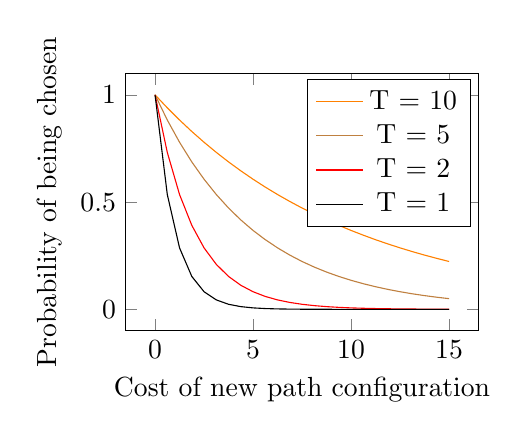
\begin{tikzpicture}
        \begin{axis}[
            width=0.5\textwidth,
            height=0.4\textwidth,
            xlabel=Cost of new path configuration,
            ylabel=Probability of being chosen
        ]
        \addplot[
            color=orange,
            domain=0:15
        ]
        {exp(-x / 10)};
        \addlegendentry{T = 10}
        \addplot[
            color=brown,
            domain=0:15
        ]
        {exp(-x / 5)};
        \addlegendentry{T = 5}
        \addplot[
            color=red,
            domain=0:15
        ]
        {exp(-x / 2)};
        \addlegendentry{T = 2}
        \addplot[
            color=black,
            domain=0:15
        ]
        {exp(-x / 1)};
        \addlegendentry{T = 1}
        \end{axis}
    \end{tikzpicture}
    \caption{Relationship between change in path cost and probability of selection}
\end{figure}

As a result, we can see that the greater the energy, the exponentially lower the probability it is chosen, however, the probability is still greater at higher temperatures.
\\

\textbf{Local Search (2 opt)}

It is an important part of the algorithm to determine an algorithm to search for nearby possible solutions.
A well known method is the \textbf{two-opt} method.
This involves selecting two random cities, re-orders the route between each other so that it does not.
\\

The example below shows before ($A \rightarrow B \rightarrow D \rightarrow C \rightarrow E \rightarrow F$) on the left, and after reversing the order between nodes B and E ($A \rightarrow B \rightarrow C \rightarrow D \rightarrow E \rightarrow F$) on the right.

\begin{figure}[!h]
    \centering
    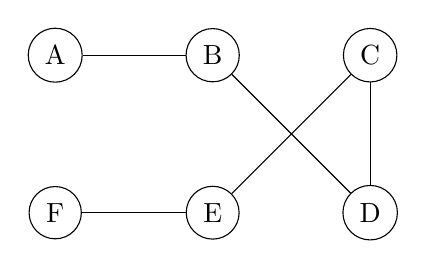
\begin{tikzpicture}
        \node[shape=circle,draw=black] (A) at (0,2) {A};
        \node[shape=circle,draw=black] (B) at (2,2) {B};
        \node[shape=circle,draw=black] (C) at (4,2) {C};
        \node[shape=circle,draw=black] (D) at (4,0) {D};
        \node[shape=circle,draw=black] (E) at (2,0) {E};
        \node[shape=circle,draw=black] (F) at (0,0) {F};
    
        \path [-](A) edge node[left] {} (B);
        \path [-](B) edge node[left] {} (D);
        \path [-](D) edge node[left] {} (C);
        \path [-](C) edge node[left] {} (E);
        \path [-](E) edge node[left] {} (F);
    \end{tikzpicture}
    \quad \quad \quad
    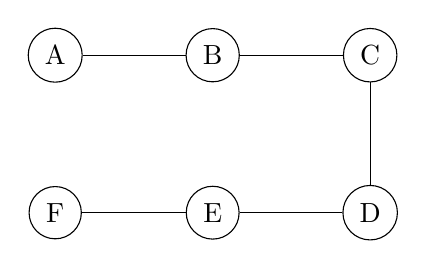
\begin{tikzpicture}
        \node[shape=circle,draw=black] (A) at (0,2) {A};
        \node[shape=circle,draw=black] (B) at (2,2) {B};
        \node[shape=circle,draw=black] (C) at (4,2) {C};
        \node[shape=circle,draw=black] (D) at (4,0) {D};
        \node[shape=circle,draw=black] (E) at (2,0) {E};
        \node[shape=circle,draw=black] (F) at (0,0) {F};
    
        \path [-](A) edge node[left] {} (B);
        \path [-](B) edge node[left] {} (C);
        \path [-](C) edge node[left] {} (D);
        \path [-](D) edge node[left] {} (E);
        \path [-](E) edge node[left] {} (F);
    \end{tikzpicture}
    \caption{two-opt between B and E}
\end{figure}

In the above scenario, the "before" distance will be shorter than the "after" distance if

$$\text{distance}(B, D) + \text{distance}(C, E) < \text{distance}(B, C) + \text{distance}(D, E)$$

which can be calculated in $O(1)$, whilst applying the two-opt runs in $O(n)$.
Hence, in the implementation, the loss of the new path configuration is calculated first before the path is changed. \\

Note that a more optimal method is the LKH (Lin–Kernighan heuristic), however, this is a largely a variation of the two-opt and three-opt method.
However, because of its difficulty in implementation \cite{helsgaun98}, and the main focus is on the temperature and cooling rate, only two-opt been implemented.

\subsection{Code}

For the implementation there are three main python files:

\begin{itemize}
    \item \texttt{src/solvers.py} 
    
    This contains classes that extend an abstract class \texttt{Solver} which contains abstract methods \texttt{get\_next\_order()} which runs one iteration of the solving algorithm, returning the current path it has found (used in the visualisation).
    It also contains the \texttt{SimulatedAnnealing} class, which takes in optional parameters \texttt{temperature} and \texttt{cooling\_rate}.
    
    \item \texttt{src/main.py} 
    
    This contains the code for running a visualisation of a problem from a file or randomly generated cities.
    It also has a method \texttt{solve()} which runs \texttt{get\_next\_order()} until the algorithm has determined that is has finished.
    
    \item \texttt{src/benchmark.py}
    
    This contains the code to benchmark the \texttt{SimulatedAnnealing} solver.
    It can either load in problems from a file or generate random problems (as detailed later in the report) and tests the \texttt{SimulatedAnnealing} solver with different options for \texttt{temperature} and \texttt{cooling\_rate}.

\end{itemize}

The \texttt{data} folder contains different problems taken from the TSPLIB library, where \texttt{.tsp} files contain problem instances, and \texttt{.opt.tour} files contain the optimal tour for the problem.

%%%%%%%%%%%%%%%%%%%%%%%%%%%%%%%%%%%%%%%%%%%%%%%%%%%%%%%%%%%%%%%%%%%%%%%%%%%%%%%%
\newpage
\section{Experimentation}

\subsection{TSP Dataset Test}
First the SA algorithm was benchmarked with TSPLIB \cite{tsplib} (a public library for TSP instances) with different initial temperatures and cooling rates.
The problems sets that were used are listed below

\begin{multicols}{6}
\begin{verbatim}
a280.tsp
att48.tsp
berlin52.tsp
ch130.tsp
ch150.tsp
gr666.tsp
pcb442.tsp
pr1002.tsp
pr2392.tsp
rd100.tsp
tsp225.tsp
ulysses22.tsp
\end{verbatim}
\end{multicols}

To conduct a test, the SA algorithm would be bench marked, with a temperature and cooling rate of 0.
Then it would be run again with different combinations of temperature and cooling rates.
All of these tests would then be repeated multiple times as each run of SA can produce very different results.
The algorithm was then determined to have "finished" after it did not find a better solution after 1000 iterations.
\\

The following variables were used:

\begin{verbatim}
TEST_REPEATS = 20
TEMPERATURES = [10, 50, 100, 500, 1000, 5000]
COOLING_RATES = [0.999, 0.9995, 0.9999, 0.99995]
\end{verbatim}

where \texttt{TEST\_REPEATS} is the number of time each test was repeated, \texttt{TEMPERATURE} is the initial temperature, and \texttt{COOLING\_RATE} is how much the temperature decreases each iteration.

\subsubsection{Results}

\begin{figure}[h]
    \centering
    \begin{tabular}{ |c|c|c|c| } 
        \hline
        Cooling Rate & Mean Optimality & Optimality Std Dev & Mean Iterations \\ 
        \hline
        0       & 0.7206 & 0.2151 & 69942 \\
        \hline
        0.999   & 0.7190 & 0.2151 & 71486 \\
        \hline
        0.9995  & 0.7214 & 0.2165 & 73394 \\ 
        \hline
        0.9999  & 0.7388 & 0.2263 & 94316 \\
        \hline
        0.99995 & 0.7549 & 0.2287 & 125381 \\
        \hline
    \end{tabular}
    \caption{Results of different cooling rates of the TSPLIB problems}
\end{figure}

\begin{figure}[h]
    \centering
    \begin{tabular}{ |c|c|c|c| } 
        \hline
        Temperature & Mean Optimality & Optimality Std Dev & Mean Iterations \\ 
        \hline
        0    & 0.7206 & 0.2151 & 69942 \\
        \hline
        10   & 0.7236 & 0.2171 & 74344 \\
        \hline
        50   & 0.7343 & 0.2207 & 81645 \\
        \hline
        100  & 0.7341 & 0.2230 & 84811 \\ 
        \hline
        500  & 0.7381 & 0.2233 & 95380 \\
        \hline
        1000 & 0.7367 & 0.2245 & 99195 \\
        \hline
        5000 & 0.7343 & 0.2245 & 111490 \\
        \hline
    \end{tabular}
    \caption{Results of different initial temperatures of the TSPLIB problems}
\end{figure}

\begin{figure}[h]
    \centering
    \begin{tabular}{ |c|c|c|c|c| } 
        \hline
        Name & City Count & Avg. City Distance & Avg. Iterations & Avg. Optimality \\ 
        \hline
        ulysses22.tsp & 22   & 4    & 84003  & 0.9991 \\
        \hline
        att48.tsp     & 48   & 1608 & 17216  & 0.9576 \\
        \hline
        berlin52.tsp  & 52   & 282  & 29205  & 0.9342 \\ 
        \hline
        rd100.tsp     & 100  & 275  & 32775  & 0.8780 \\
        \hline
        ch130.tsp     & 130  & 177  & 39815  & 0.8576 \\
        \hline
        ch150.tsp     & 150  & 178  & 40381  & 0.8087 \\
        \hline
        tsp225.tsp    & 225  & 91   & 56350  & 0.7502 \\
        \hline
        a280.tsp      & 280  & 61   & 68501  & 0.6757 \\
        \hline
        pcb442.tsp    & 442  & 872  & 78402  & 0.5924 \\
        \hline
        gr666.tsp     & 666  & 44   & 133338 & 0.6904 \\
        \hline
        pr1002.tsp    & 1002 & 3215 & 156407 & 0.4064 \\
        \hline
        pr2392.tsp    & 2392 & 3186 & 347207 & 0.2458 \\
        \hline
    \end{tabular}
    \caption{Results of different TSPLIB problems}
\end{figure}

\begin{figure}[H]
\centering
    \begin{subfigure}{0.45\textwidth}
        \centering
        \includegraphics[width=1\linewidth]{images/tsplib_optimality_city_count.jpg}
        \caption{Cooling temp optimality for city count}
        \label{fig:sub1}
    \end{subfigure}%
    \begin{subfigure}{0.45\textwidth}
        \centering
        \includegraphics[width=1\linewidth]{images/tsplib_optimality_cooling_rate.jpg}
        \caption{Optimality for each cooling rate}
        \label{fig:sub2}
    \end{subfigure}
    \caption{Visualisation between optimality, city counts, and cooling rate}
\end{figure}


\begin{figure}[H]
\centering
    \begin{subfigure}{0.45\textwidth}
        \centering
        \includegraphics[width=1\linewidth]{images/tsplib_optimality_city_dist.jpg}
        \caption{Temp optimality for city distance}
        \label{fig:sub1}
    \end{subfigure}%
    \begin{subfigure}{0.45\textwidth}
        \centering  
        \includegraphics[width=1\linewidth]{images/tsplib_optimality_temperature.jpg}
        \caption{Optimality for each initial temperature}
        \label{fig:sub2}
    \end{subfigure}
    \caption{Visualisation between optimality, city distances and temperatures}
\end{figure}

\subsubsection{Discussion}

From these results there are a couple observations that we can make
\begin{itemize}
    \item There is a negative exponential correlation between city count and temperature, however, there was a lack of correlation between city distance and optimality
    \item The higher the cooling rate, the better the optimality, however, there is no benefit to constantly increasing the temperature
    \item There was a logarithmic trend between cooling rate and iterations, and also a logarithmic trend between initial temperature and iterations
\end{itemize}

However, there are also issues that need to be addressed
\begin{itemize}
    \item gr666.tsp is an outlier, is a dense cluster of cities, whilst the rest are sparsely scattered, resulting in a higher average optimality as despite perhaps having a bad path configuration - because so many cities were close, the change in distance was small)
    \item since optimality has a very small correlation with optimality, we cannot tell if a certain temperature increases the optimality for an average city distance unless there is the same number of cities
\end{itemize}

To get more meaningful results, there needed to be a greater increase in the range of the cooling rate to determine the limit of a higher cooling rate.
The problem set used for the TSP problem also needs to be better controlled, as the impact of temperature on optimality for different temperatures could not be determined as optimality was more dependent on the number of cities.

\subsection{Random Dataset Test}
In this new test, rather than using TSPLIB problems, our own data will be produced randomly, where we can vary or keep constant variables such as the city count and distance.
\\

To generate the problem instances, the following variables were used

\begin{verbatim}
MAP_SIZES = [50, 100, 500, 1000, 1500]
CITY_COUNTS = [50, 100, 500, 1000, 1500]
CONST_CITY_COUNT = 100
CONST_MAP_SIZE = 100
\end{verbatim}

where \texttt{MAP\_SIZES} was the maximum value that an x or y coordinate of a city could take, and \texttt{CITY\_COUNT} was the number of cities in a map.

To generate the random problem set, the \texttt{CONST\_CITY\_COUNT} would be used to generate a problem with the other map sizes.
Then \texttt{CONST\_MAP\_SIZE} would be used to generate a problem with the other city counts.
This would then result in 10 different maps.
\\

Then for testing, the a different temperature would be used to 
\\

While the following variables from the original test were changed to be:

\begin{verbatim}
RAND_TEST_REPEATS = 20
RAND_TEMPERATURES = [10, 50, 100, 500, 1000]
RAND_COOLING_RATES = [0.999, 0.9995, 0.999_9, 0.999_95, 0.999_99]
RAND_CONST_TEMPERATURE = 10
RAND_CONST_COOLING_RATE = 0.999
\end{verbatim}

\subsubsection{Results}

\subsubsection{Discussion}

%%%%%%%%%%%%%%%%%%%%%%%%%%%%%%%%%%%%%%%%%%%%%%%%%%%%%%%%%%%%%%%%%%%%%%%%%%%%%%%%
\newpage
\section{Conclusion}



%%%%%%%%%%%%%%%%%%%%%%%%%%%%%%%%%%%%%%%%%%%%%%%%%%%%%%%%%%%%%%%%%%%%%%%%%%%%%%%%
\newpage
\section{References}
\bibliographystyle{standard}
\begin{thebibliography}{9}

\bibitem{cook12}
Cook, William J. (2012) \emph{In Pursuit of the Traveling Salesman: Mathematics at the Limit of Computation.} Princeton, NJ: Princeton UP

\bibitem{helsgaun98}
K. Helsgaun, (1998) \emph{An Effective Implementation of the Lin-Kernighan Traveling Salesman Heuristic. DATALOGISKE SKRIFTER (Writings on Computer Science), No. 81} Roskilde University.

\bibitem{tsplib}
G. Reinelt, (1991) \emph{TSPLIB - A Traveling Salesman Problem Library”,} ORSA J. Comput., 3-4, 376-385.

\bibitem{cooling}
Mahdi, Walid \& Medjahed, Seyyid Ahmed \& Ouali, Mohammed. (2017) \emph{Performance Analysis of Simulated Annealing Cooling Schedules in the Context of Dense Image Matching.} Computación y Sistemas. 21. 493-501. 10.13053/CyS-21-3-2553. 
\end{thebibliography}

\end{document}
